\subsection{Finding \texorpdfstring{$T_{1}$}{T1} for Water, Ethanol and Rubber Using Saturation Recovery Sequence} \label{B3}

With a 90$\degree$-$\tau$-90$\degree$ pulse sequence, the  magnetic vector regrowth along the $z$-axis is given by equation \ref{eqn:SR},
\begin{align*}
M_z(t) &= M_0(1 - e^{-\tau/T_1} ) \\
\intertext{As the second pulse has been set to have $M_z=M_0/2$, }
\frac{1}{2} &= 1 - e^{-\frac{\tau}{T_{1}}}
\end{align*}
Taking the natural logarithm of both sides and rearranging,
\begin{align*}
T_1 &= \frac{\tau}{\ln 2} \numberthis \label{eqn:B3:T1}
\end{align*}

The time delay between the two pulses, $\tau$, was measured in post-processing by calculating the peaks in of the digital oscilloscope trace data. $\tau$ was set such that, 
\[ M_z\approx M_0/2 \numberthis \label{eqn:B3:M0/2} \]

As the determination of what time delay $\tau$ satisfies Equation \ref{eqn:B3:M0/2} is approximate at best, three data traces were saved and analyzed in post-processing. The three data sets spanned the approximate range of time delays, such that the data sets have peak magnetization of $\lesssim M_0/2$, $\approx M_0/2$ and $\gtrsim M_0/2$. A simple 90$\degree$ FID (as in Section \ref{B1}) was used to calculate a $M_0/2$ in post-processing. A linear slope was fit between the time-delayed peaks of the three approximate data sets (see Figure \ref{fig:B3:example_uncertainty}) and the point on this slope where $M_z = M_0/2$ is our calculated value of $\tau$. $T_1$ is then computed using Equation \ref{eqn:B3:T1}. As there is a large number of error in this measurement caused by uncertainty in the measurement of $M_0$, the peak detection on the saturation recovery peaks, and the linear fit, the uncertainty is taken to encompass the recovery peaks in all three traces. It could be an improvement to take more than three data points to create the line but this is a rough approximation so additional data points were not taken.

%there is large error in the measurement as the recording of $M_0$ was approximated to begin with and measuring half that data is also approximate. So, to determine an uncertainty in $\tau$, three traces were saved in the range of $\tau$ which satisfied Equation \ref{eqn:B3:M0/2} -- one at the lower end, center, and high end. The final value is taken as the mean of the the three $\tau_i$ values, and the uncertainty determined as the minimum value to encompass all three measured values. Mathematically, if the three measure time delays are denoted as $\tau_i$ where $i=1,2,3$, then the final value is,


\begin{figure}[H]
    \centering
    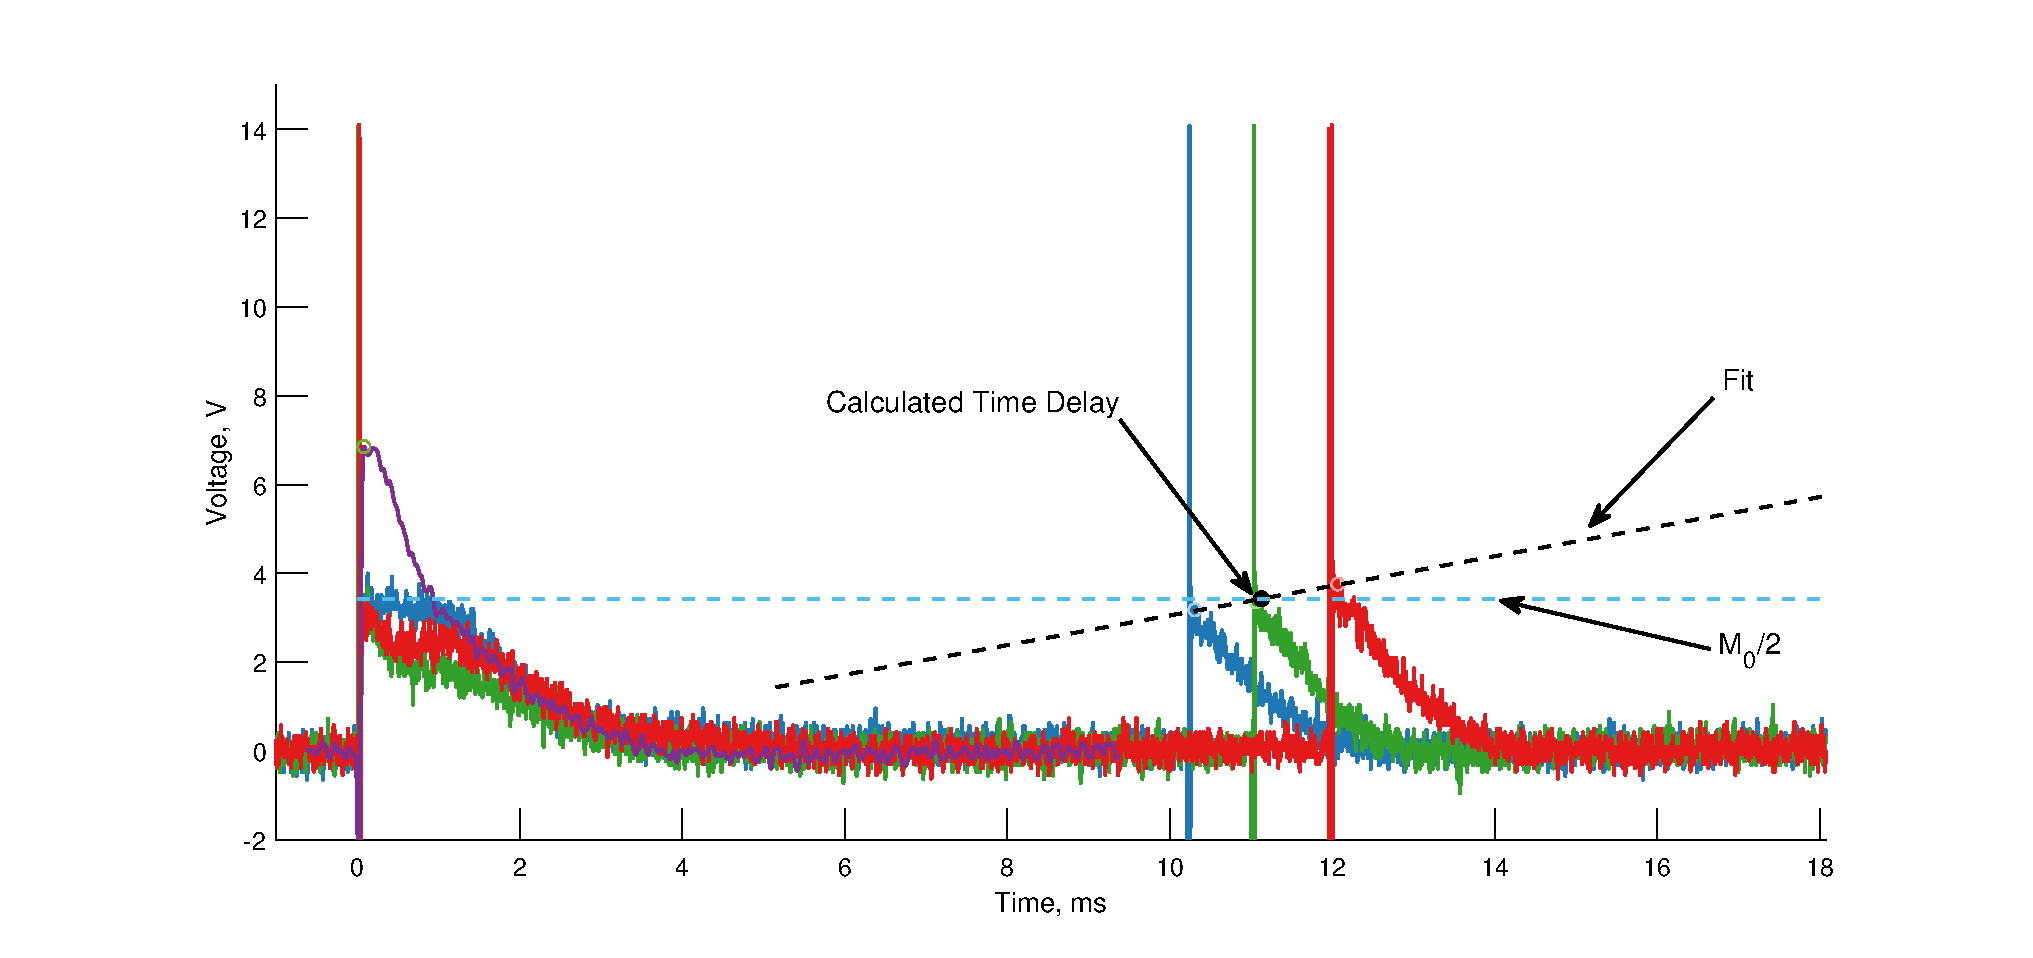
\includegraphics[width=\textwidth]{figures/B3/B3_2.eps}
    \caption{Three doped water saturation recovery traces with $\tau \approx M_0/2$, as well as 90 degree FID (purple trace) to measure $M_0$ with greater precision. Calculated $\tau$ value is shown as black circle and linear fit is dotted black line.}
    \label{fig:B3:example_uncertainty}
\end{figure}

This process was repeated for ethanol and rubber, and the calculated $T_1$ values are tabulated in Table \ref{tab:B3:T1values}.

\begin{table}[H]
    \centering
    \begin{tabular}{c|c}
    \toprule
        \textbf{Sample} & $T_1$ (ms) \\ \midrule
        {Doped Water} & $16.2770  \pm  1.1537$ \\
        {Ethanol} & $1029.1 \pm 80.1$  \\
        {Rubber} & $34.1179 \pm 5.658$ \\ \bottomrule
    \end{tabular}
    \caption{$T_1$ values for three samples, measured using a saturation recovery pulse sequence.}
    \label{tab:B3:T1values}
\end{table}

A second method for estimating $T_1$ can be performed during this experiment. While probing the sample with a 90$\degree$ FID sequence, the signal will decrease rapidly when the repetition rate is approximately equal to $5T_1$. By reducing the pulse repetition rate until no signal is visible, the previous repetition rate is a highly approximated value of $5T_1$. This estimation of $T_1$ is highly imprecise as there is only 5 options for pulse repetition rate with large space between them. Thus, the `resolution' of this method is very low. The calculated time constant would always be greater than its true value, as the last setting \textit{prior} to the signal decrease is used as the estimate. This method was not performed, but could be useful for gaining insight into the order of magnitude and an upper bound for $T_1$.  \\

%To experimentally get the time \textit{t} for which $M(t) = \frac{M_0}{2}$, two 90 degree pulses were applied to the signal and the time was adjusted until the amplitude of the signal equaled $\frac{M_0}{2}$. The time difference between the two pulses is equal to \textit{t} for the $T_1$ calculation above. The two pulses can be identified as the spikes in the graph below:
%\begin{figure}[H]
%\centering
%\label{FIDApprxT1}
%\includegraphics[width=0.6\textwidth]{WaterT1.jpg}
%\caption{FID graph for water illustrating $T_{1}$ approximation.}
%\end{figure}
%From the graph above, we can see that the time difference used to calculate $T_1$ is equal to 0.017244 s. Therefore, using the $T_1$ equation above:
%From this approximation we can see that $T_1$ for water was an order of magnitude larger than $T_{2}^*$.The $T_1$ uncertainty for this method is  hard to approximate 